\chapter{Propuesta}\label{chapter:proposal}

Existen varios sistemas automatizados de respuesta a preguntas, pero son de propósito general, por lo que habría que entrenar sus modelos del lenguaje con datos sobre la facultad \textit{MATCOM}, y ahora mismo no se tienen esos datos, y tampoco la infraestructura necesaria para llevar a cabo un proyecto de tales magnitudes, por lo que es más factible optar por un sistema manual o híbrido.
\newline

Por otra parte, los sistemas manuales/híbridos que existen en el mercado, o son de pago, o no se acogen estrictamente a las necesidades de la facultad, además de que se contempla en un futuro integrar este sistema con otros proyectos, y para ello es necesario que este sea totalmente personalizable.
\newline

Es preciso que sea un proyecto web, por la facilidad que estos brindan de ser usados en cualquier lugar y dispositivo.
\newline

El sistema tendrá las siguientes características:
\newline

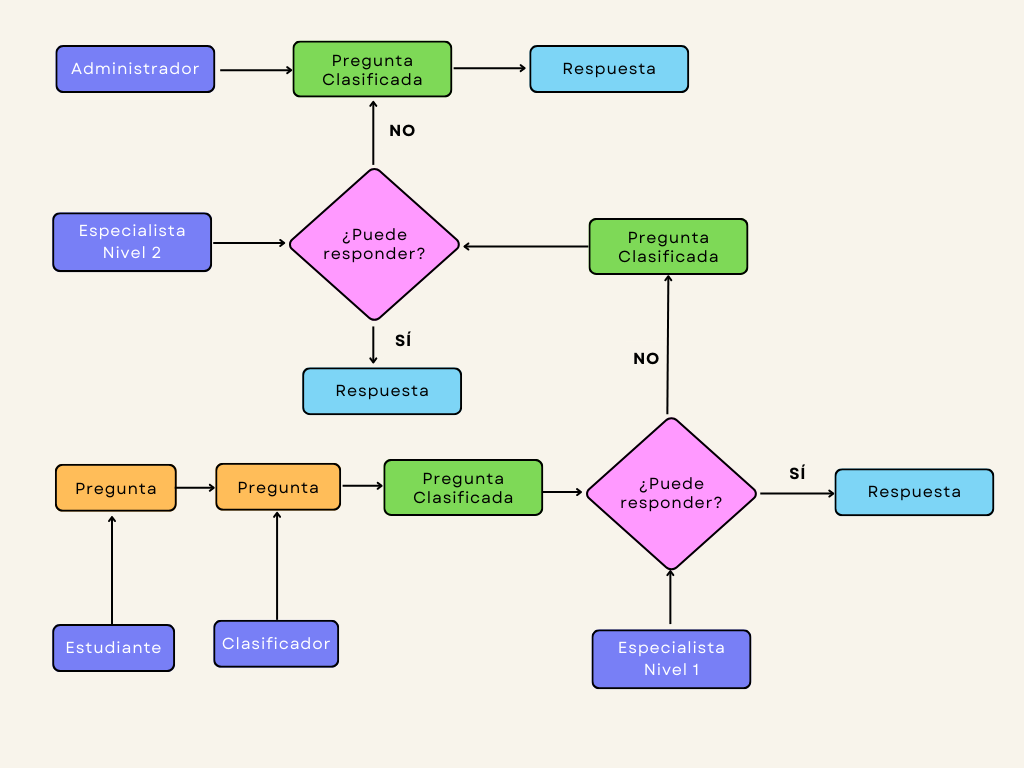
\includegraphics[width=15cm, height=11.25cm]{thesis_diagram.png}

\begin{itemize}
	\item Los usuarios se deben poder crear una cuenta en la plataforma con la cual iniciar sesión.
	
	\item Los usuarios se deben dividir en 5 roles: estudiante, clasificador, administrador, especialista de nivel 1 y especialista de nivel 2.
	
	\item Los estudiantes deben ser capaces de escribir sus dudas, ver su historial de dudas con sus respectivas respuestas y, por cada duda, deben poder abrir un chat con los responsables de darle respuesta.
	
	\item Los clasificadores deben ser capaces de ver las dudas sin clasificar, y deben poder clasificarlas eligiendo un área de un conjunto previamente creado por el administrador.
	
	\item Los administradores deben poder crear áreas en las cuales se clasificarán las preguntas, pueden responder cualquier pregunta independientemente del área en que haya sido clasificada, asignarle áreas a los especialistas de nivel 1 y nivel 2, ver la información de los usuarios registrados en el sistema, cambiar de rol a cualquier usuario y, por cada duda, chatear con el estudiante autor de la misma.
	
	\item Los especialistas de nivel 1 deben pertenecer al área que el administrador haya decidido, deben ver el listado de preguntas clasificadas en su área, responder dichas preguntas, subir la pregunta de nivel en el caso de no poder responderla, y, por cada duda, chatear con el estudiante autor de esta.
	
	\item Los especialistas de nivel 2 deben pertenecer al área que el administrador haya decidido, deben ver el listado de las preguntas clasificadas en su área que hayan sido subidas de nivel por algún especialista de nivel 1, deben poder responder dichas preguntas, subir a la administración las dudas que no sean capaces de responder, y, por cada duda, chatear con el estudiante autor de esta.
\end{itemize}

De esta manera se garantiza de que cada pregunta va a llegar a la persona capacitada para darle respuesta, y con este flujo y el personal adecuado se puede garantizar que los estudiantes resuelvan su duda en el menor tiempo posible.